\section{一维问题}
\label{sec:one_dim}

本章我们将讨论两个最为简单的一维问题:无限深方势阱与谐振子问题。

% =================================================
\subsection{无限深方势阱}
\label{subsec:onedim_inf_square}

现在我们讨论一个一维粒子,其位于一个无限深的方形势阱中:
\begin{equation}
    V(x) =
    \begin{cases}
        \infty, & x<0,  \\
        0,      & 0<x<a,\\
        \infty, & x>a.  \\
    \end{cases}
\end{equation}
一般的任务即为求解该系统的能级分布(可能的本征能量)或某个特定量子态的力学量平均值。
这里,势能的形状使得在坐标表象下求解较为方便。

下面求解系统的能级。

首先写出体系的Hamiltonian量
\begin{equation}
    H = \frac{p^2}{2m} + V(x),
\end{equation}
在坐标表象下,Hamiltonian算符的形式为
\begin{equation}
    H = -\frac{\hbar^2}{2m} \pd_{xx}^2 + V(x),
\end{equation}

体系是不含时的,因此能量是守恒量,一个普遍的量子态可以表为诸能量本征态与时间相位的乘积:
\begin{equation}
    \psi(x,t) = \sum_n \psi_{E_n}(x) \ee^{-\ii E_n t/\hbar},
\end{equation}
而$\psi_{E_n}(x)$是能量本征方程
\begin{equation}
    H\psi(x) = E \psi(x)
\end{equation}
的本征值为$E=E_n$的解。

下面求解能量本征方程。
能量本征方程是一个常微分方程,其中$V(x)$是分段的,因此需要分段讨论,做法是分别在各段上求取含参数的通解,并在各段交界处通过边界条件衔接,确定参数。
因此我们在(1) $x<0$; (2) $x>a$; (3) $0<x<a$三段区间上讨论。

(1) (2) 我们注意到,在这两段上,$V(x)=\infty$,因此粒子决不可能在上面存在任意的概率分布,否则能量平均值也将趋于$\infty$,因此这两段上$\psi(x)=0$。

(3) 在这一段上,$V(x)=0$,能量本征方程化为
\begin{equation}
    -\frac{\hbar^2}{2m} \pd_{xx}^2 \psi(x) = E \psi(x).
\end{equation}
我们置$k\coloneq \sqrt{2mE}/\hbar$\footnote{事实上,按de Broglie关系,这里的$k=p/\hbar$正是具有动量$p$本征态的波函数的波矢大小。},方程化为$(\pd_{xx}^2+k^2) \psi(x) = 0$,解得
\footnote{当然,也可以$\psi(x)=A\exp(\pm\ii k x)$作为两个线性无关解,之后进行线性组合得到符合边界条件的解即可,不过显然,取两个实函数总是更方便的。}
\begin{equation}
    \psi_{1,k}(x) = A_{1,k} \sin kx ,\quad \psi_{2,k}(x) = A_{2,k} \cos kx,
\end{equation}
其中$k$是参数。

接下来我们考察解的衔接问题:在$x=0, x=a$处,均要求$\psi(x)=0$。
这便要求在第(3)段解得的波函数满足$\psi(0)=\psi(a)=0$。
我们首先考察两组参数为$k$的解:
$\psi_{2,k}(x)$对于任意$k$始终无法满足$\psi(0)=0$,故舍去该组解。
对于$\psi_{1,k}(x)$,其对任意$k$始终满足$\psi(0)=0$;而对于条件$\psi(a)=0$,仅有离散的$k$取值$k_n=n\pi/a$使得波函数满足条件。
于是,我们最终确定了能量本征方程的解:
\begin{equation}
    \psi_n(x) =
    \begin{cases}
        0,                          & (x<0)\vee(x>a),  \\
        A_n \sin\frac{n\pi x}{a},   & 0 \leq x \leq a.\\
    \end{cases}
\end{equation}
这些能量本征函数以$n$标号,对应$k_n=n\pi/a$,有对应的本征能量
\begin{equation}
    E_n = \frac{\hbar^2 k_n^2}{2m} = \frac{n^2 \pi^2 \hbar^2}{2m a^2}.
\end{equation}

我们还需进一步确定本征波函数的归一化系数$A_n$,这一系数由总概率为1确定:
\begin{equation}
    P = \braket{\psi}{\psi} = 1,
\end{equation}
得$A_n = \sqrt{2/a}$。

现在,我们完全确定了系统的能量本征态及其对应的本征能量
\footnote{需要注意的是,在实际应试中,永远不应该直接照搬这一结论,因为势阱的位置和宽度均可能有变化,因此,按照这里的思路随机应变求解是最稳妥的。}
\begin{equation}
    \psi_{E_n} = \sqrt{\frac2a} \sin\frac{n\pi x}{a} ,\quad E_n = \frac{n^2 \pi^2 \hbar^2}{2m a^2}, \quad n=1,2,\cdots.
\end{equation}

注意:记忆能级不靠背诵,利用$p=\hbar k$,$k_n=n\pi/a$及$E=p^2/2m$即可定出能级。

\begin{figure}[ht]
    \centering
    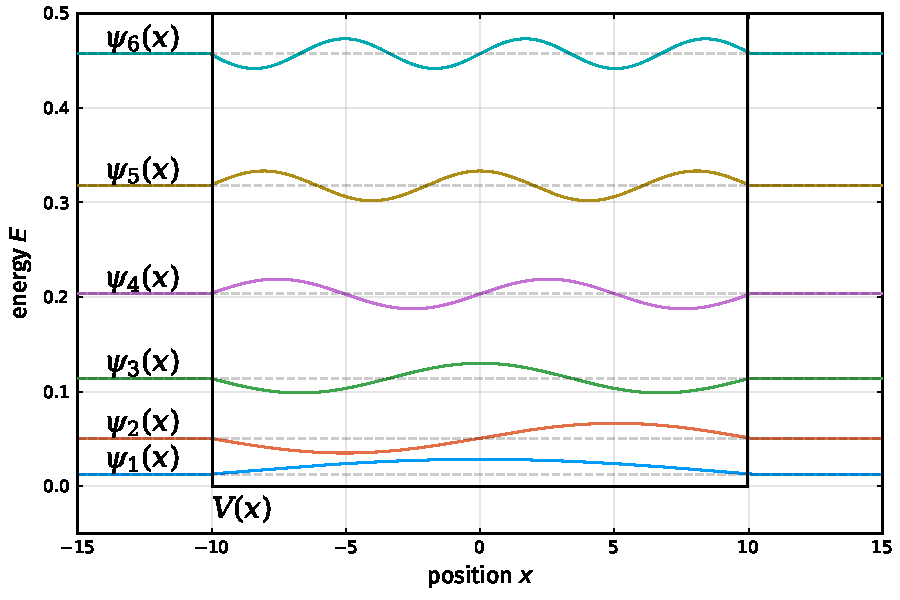
\includegraphics[width=0.8\textwidth]{figures/sec3_figures/infinite_well_eigenstates.pdf}
    \caption{无限深方势阱的能量本征态。}
\end{figure}

若已知系统零时刻处于几个能量本征态的叠加态,要求解系统波函数随时间的演化,将零时刻波函数投影至这些能量本征波函数之后,分别乘以相应的时间相位$\exp(-\ii E t/\hbar)$,重新相加即可。
一个运算技巧是先不要急于代入能量的表达式,而是先表为$E_n=n^2 E_1$,在化简完毕后再代入$E_1$的表达式。

若要求解系统的力学量平均值,直接使用相应算符在坐标表象下的表式求解即可,例如,坐标平均值
\begin{equation}
    \expval{x} = \mel{\psi}{x}{\psi} = \int_0^a \psi^*(x) \cdot x \psi(x) = \int_0^a x \abs{\psi(x)}^2;
\end{equation}
动量平均值
\begin{equation}
    \expval{p} = \mel{\psi}{p}{\psi} = \int_0^a \psi^*(x) \cdot -\ii\hbar\pd_x \psi(x);
\end{equation}
动量平方平均值
\begin{equation}
    \expval{p^2} = \mel{\psi}{p^2}{\psi} = \int_0^a \psi^*(x) \cdot -\hbar^2\pd_{xx}^2 \psi(x).
\end{equation}
注意,不少情况下,利用波函数的对称性及不同能级波函数的正交性可简化计算。

在计算的时候,也应熟记一些与三角函数有关的推论,例如二倍角与积化和差公式:
\begin{itemize}
    \item 二倍角公式
    \begin{equation}
    \begin{aligned}
        \sin 2\alpha &= 2\sin\alpha\cos\alpha, \\
        \cos 2\alpha &= \cos^2\alpha - \sin^2\alpha = 2\cos^2\alpha - 1 = 1 - 2\sin^2\alpha.
    \end{aligned}
    \end{equation}
    \item 积化和差公式
    \begin{equation}
    \begin{aligned}
        2\cos\alpha\cos\beta &= \cos(\alpha-\beta) + \cos(\alpha+\beta), \\
        2\sin\alpha\sin\beta &= \cos(\alpha-\beta) - \cos(\alpha+\beta), \\
        2\sin\alpha\cos\beta &= \sin(\alpha+\beta) + \sin(\alpha-\beta).
    \end{aligned}
    \end{equation}
\end{itemize}


% =================================================
\subsection{一维谐振子}
\label{subsec:onedim_osc}

我们设质量为$m$的物体受到$F=-kx$的弹性回复力,构成一维谐振子。

取平衡位置为原点,并利用圆频率$\omega\coloneq\sqrt{k/m}$,我们得到势能表式
\begin{equation}
    V(x) = \frac12 kx^2 = \frac12 m\omega^2 x^2,
\end{equation}
并进一步得到体系的Hamiltonian量
\begin{equation}
    \label{eq:onedim_osc_ham}
    H = \frac{p^2}{2m} + \frac12 m\omega^2 x^2.
\end{equation}

% ================================
\subsubsection{坐标表象}

在坐标表象下,可以写出一维谐振子的能量本征方程
\begin{equation}
    \left[ -\frac{\hbar^2}{2m}\pd_{xx}^2 + \frac12 m\omega^2 x^2 \right] \psi(x) = E\psi(x).
\end{equation}

作变量代换$\xi\coloneq \sqrt{m\omega/\hbar} x \coloneq \alpha x$,$\lambda = E/(\hbar\omega/2)$,
并作函数代换$\psi(\xi)=u(\xi)\ee^{-\xi^2/2}$,可得$u(\xi)$满足Hermite方程
\begin{equation}
    u''-2\xi u'+(\lambda-1)u = 0,
\end{equation}
可得满足波函数无穷远处渐近行为($\psi(x)\rightarrow 0$)的解为$u_n(\xi) = \rm{H}_n(\xi)$,
这里$\rm{H}_n(\xi)$是Hermite多项式,
对应的$\lambda=2n+1, n=0,1,2,\cdots$。

\begin{tcolorbox}
于是,就得到了一维谐振子体系的归一化能量本征函数及其对应的能量本征值:
\begin{equation}
    \label{eq:onedim_osc_coord_wfn}
    \psi_n(x) = \sqrt{\frac{\alpha}{2^n\cdot n! \sqrt{\pi}}} \rm{H}_n(\alpha x) \ee^{-\alpha^2 x^2/2}, \quad n=0,1,2,\cdots
\end{equation}
\begin{equation}
    E_n = \left(n+\frac12\right) \hbar\omega.
\end{equation}

特别地,对于基态,有
\begin{equation}
    \psi_0(x) = \sqrt{\frac{\alpha}{\sqrt{\pi}}} \ee^{-\alpha^2 x^2/2},
\end{equation}
\begin{equation}
    E_0 = \frac12 \hbar\omega.
\end{equation}
\end{tcolorbox}

\begin{figure}[ht]
    \centering
    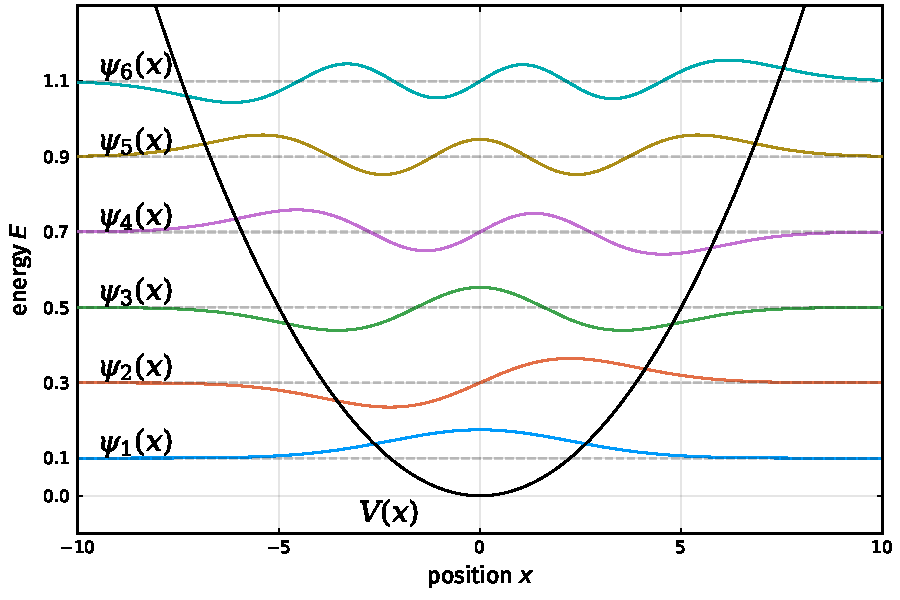
\includegraphics[width=0.8\textwidth]{figures/sec3_figures/harmonic_oscillator_eigenstates.pdf}
    \caption{一维谐振子的能量本征态。}
\end{figure}


% ================================
\subsubsection{粒子数表象}

我们注意到式\eqref{eq:onedim_osc_ham}中的坐标与动量算符的阶数均为二次,是对称的。
因此可以由此出发构建一组新的坐标,在新的表象下研究谐振子问题。

我们引入无量纲算符
\begin{equation}
    Q \coloneq \sqrt{\frac{m\omega}{\hbar}} x ,\quad P \coloneq \sqrt{\frac{1}{m\hbar\omega}} p,
\end{equation}
其对易子$[Q,P]=\ii$,
这样,Hamiltonian算符成为
\begin{equation}
    H = \frac12 \hbar\omega (Q^2+P^2).
\end{equation}

现我们定义算符
\begin{equation}
    a \coloneq \frac{1}{\sqrt{2}} (Q+\ii P) ,\quad a^\dag \coloneq \frac{1}{\sqrt{2}} (Q-\ii P),
\end{equation}
其对易子$[a,a^\dag]=1$。
我们发现
\begin{equation}
    a^\dag a = \frac12 (Q-\ii P)(Q+\ii P) = \frac{1}{\hbar\omega} H - \frac12,
\end{equation}
这就是说,
\begin{equation}
    H = (a^\dag a+\frac12)\hbar\omega.
\end{equation}
由$[a,a^\dag]=1$立刻得到
\begin{equation}
    H = (a a^\dag-\frac12)\hbar\omega
\end{equation}

我们假设谐振子按能量从低到高的第$n$($n=0,1,\cdots$)个能量为$E_n$的能量本征态为$\ket{n}$,然后考察$a,a^\dag$算符对能量本征态的影响。

我们研究$a\ket{n}$的能量本征值:
\begin{equation}
\begin{aligned}
    H a \ket{n}
    &= (a a^\dag - \frac12)\hbar\omega \cdot a \ket{n} \\
    &= (a a^\dag a - \frac12 a)\hbar\omega \ket{n} \\
    &= a (a^\dag a - \frac12)\hbar\omega \ket{n} \\
    &= a [(H-\hbar\omega) \ket{n}] \\
    &= (E_n-\hbar\omega) a \ket{n},
\end{aligned}
\end{equation}
可知$a\ket{n}$是$H$的另一个本征态,即能量本征值为$E_n-\hbar\omega$的能量本征态。
对能量本征态作用$a$一次,谐振子的能级下降$\hbar\omega$,因此$a$称为\emph{降算符}。
但能量不能无限下延,必须有基态能量$E_0$及对应本征态$\ket{0}$,使得$a\ket{0}$不再是本征态,为此我们可以置
\begin{equation}
    a \ket{0} = \bm{0}.
\end{equation}
借此,我们还可以求得基态能级:
\begin{equation}
    H\ket{0}
    = (a^\dag a+\frac12)\hbar\omega \ket{0}
    = \frac12\hbar\omega \ket{0}.
\end{equation}
这是说基态能级
\begin{equation}
    E_0 = \frac12 \hbar\omega.
\end{equation}

用类似的方法可以得到结论:$a^\dag\ket{n}$也是能量本征态,其能量本征值为$E_n+\hbar\omega$。
可见对能量本征态作用$a^\dag$将使得能级上升$\hbar\omega$,因此$a^\dag$称为\emph{升算符}。

在一些物理问题中,谐振子间传递的一份份能量可以看作一种称为声子的准粒子,能级的升降就对应着声子的创生和湮灭。
在量子光学中,电磁场量子化的结果是光子图像,光子的产生和湮灭也可以用升降算符表达。
因此,升/降算符又称\emph{产生(creation)/湮灭(annihilation)算符}。
另外,我们注意到$a^\dag a\ket{n}=\left(\frac{1}{\hbar\omega}H-\frac12\right)\ket{n}=n\ket{n}$,这就是说,算符
\begin{equation}
    N \coloneq a^\dag a
\end{equation}
对$\ket{n}$的本征值恰为量子数$n$,这一算符因此称为量子数/粒子数算符。
这也是这一表象名称(粒子数表象/Fock表象)的由来。

综上我们得到一维谐振子的全部能谱:
\begin{equation}
    E_n = \left(n+\frac12\right) \hbar\omega ,\quad n=0,1,2,\cdots.
\end{equation}

需要注意的是,$a$并非保留内积的幺正算符,因此$a\ket{n}\neq\ket{n-1}\ (n>0)$,而是$\lambda_n\ket{n-1}$。
通过归一条件$\braket{n}{n}=\braket{n-1}{n-1}=1$我们有
\begin{equation}
    \lambda_n^2 \braket{n-1}{n-1} = \mel{n}{a^\dag a}{n} = \mel{n}{\left(\frac{1}{\hbar\omega}H-\frac12\right)}{n} = n \braket{n}{n},
\end{equation}
于是我们得到$\lambda_n=\sqrt{n}$,进而
\begin{equation}
    a\ket{n} = \sqrt{n}\ket{n-1}.
\end{equation}
同理有
\begin{equation}
    a^\dag \ket{n} = \sqrt{n+1}\ket{n+1}.
\end{equation}
于是
\begin{equation}
\begin{aligned}
    \ket{1} &= a^\dag \ket{0}, \\
    \ket{2} &= \frac{1}{\sqrt{2}} (a^\dag)^2 \ket{0}, \\
    \ket{3} &= \frac{1}{\sqrt{3\cdot 2}} (a^\dag)^3 \ket{0}, \\
    \cdots \cdots \\
    \ket{n} &= \frac{1}{\sqrt{n!}} (a^\dag)^n \ket{0}.
\end{aligned}
\end{equation}

粒子数表象可以变换到坐标表象,从而求出谐振子的波函数。
写出升降算符在坐标表象中的表示
\begin{equation}
\begin{aligned}
    a       &= \frac{1}{\sqrt{2}}(Q+\ii P) = \frac{1}{\sqrt{2}}\left(\alpha x + \frac{1}{\alpha}\frac{\pd}{\pd x} \right), \\
    a^\dag  &= \frac{1}{\sqrt{2}}(Q-\ii P) = \frac{1}{\sqrt{2}}\left(\alpha x - \frac{1}{\alpha}\frac{\pd}{\pd x} \right).
\end{aligned}
\end{equation}
由$a\ket{0}=\bm{0}$在坐标表象下的表示
\begin{equation}
    a\ket{0} = \frac{1}{\sqrt{2}}\left(\alpha x + \frac{1}{\alpha}\frac{\pd}{\pd x} \right) \psi_0(x) = 0
\end{equation}
可以定出基态波函数,并利用归一化条件,可得
\begin{equation}
    \psi_0(x) = \sqrt{\frac{\alpha}{\sqrt{\pi}}} \ee^{-\alpha^2 x^2/2}.
\end{equation}
激发态波函数可以通过
\begin{equation}
    \ket{n} = \frac{1}{\sqrt{n!}} (a^\dag)^n \ket{0}
\end{equation}
定出,在坐标表象下,可得
\begin{equation}
    \psi_n(x) = \sqrt{\frac{\alpha}{2^n\cdot n! \sqrt{\pi}}} \left( \alpha x + \frac{1}{\alpha}\frac{\pd}{\pd x} \right)^n \ee^{-\alpha^2 x^2/2},
\end{equation}
如果我们引入$\xi=\alpha x$,并利用Hermite多项式满足的性质
\begin{equation}
    \rm{H}_n(\xi) = \ee^{\xi^2/2} \left( \xi + \frac{\pd}{\pd \xi} \right)^n \ee^{-\xi^2/2},
\end{equation}
我们就得到了坐标表象中的波函数(式\eqref{eq:onedim_osc_coord_wfn}),殊途同归。
